\documentclass[12pt,letterpaper,margin=1in]{article}
% \documentclass[twocolumn]{aastex61}

% to-do list
% ----------
% - Add items here.

% style notes
% -----------
% - This file generates by Makefile; don't be typing ``pdflatex'' or some bullshit.
% - Line break between sentences to make the git diffs readable.
% - Use \, as a multiply operator.
% - Reserve () for function arguments; use [] or {} for outer shit.
% - Use \sectionname not Section, \figname not Figure, \documentname not Article or Paper or paper.
% - Use "comoving" instead of "co-moving".
% - Use "phase space" not "phase-space", "phase-space coordinates" not "phase space coordinates".
% - Write elements as \elem{X}.

% packages
\usepackage[letterpaper,margin=1in]{geometry}

\usepackage{setspace}
\onehalfspacing
\usepackage{microtype}  % ALWAYS!
\usepackage{amsmath,amssymb}
\usepackage[sort&compress,super]{natbib}
\usepackage{graphicx}
\graphicspath{{figures/}}
\usepackage{aas_macros}
\usepackage{hyperref}
\hypersetup{backref,breaklinks,colorlinks,citecolor=blue}
\usepackage{mathptmx}

%\setcitestyle{super}
\citestyle{nature}
\bibliographystyle{naturemag}

% define macros for text
\newcommand{\project}[1]{\textsl{#1}}
\newcommand{\acronym}[1]{{\small{#1}}}
\newcommand{\gaia}{\project{Gaia}}
\newcommand{\rave}{\project{\acronym{RAVE}}}
\newcommand{\apogee}{\project{\acronym{APOGEE}}}
\newcommand{\tmass}{\project{\acronym{2MASS}}}
\newcommand{\documentname}{Article}
\newcommand{\sectionname}{Section}
\newcommand{\figname}{Figure}
\newcommand{\eqname}{Equation}
\newcommand{\dr}{\acronym{DR1}}
\newcommand{\tgas}{\acronym{TGAS}}
\newcommand{\etal}{\textit{et al}.}
\newcommand*\elem[1]{\ensuremath{\mathrm{#1}}}
\newcommand*\elemH[1]{\ensuremath{[\mathrm{#1}/\elem{H}]}}
\newcommand*\teff{\ensuremath{T_\mathrm{eff}}}
\newcommand*\logg{\ensuremath{\log{g}}}
\newcommand*{\feh}{\ensuremath{\elemH{Fe}}}
\newcommand{\sunanalog}{\text{Krios}}
\newcommand{\bizarreone}{\text{Kronos}}
\newcommand{\Tcondens}{\ensuremath{T_C}}
\newcommand{\mearth}{\ensuremath{M_\oplus}}
\newcommand{\mjupiter}{\ensuremath{M_\mathrm{Jup}}}

% define macros for math
\newcommand{\given}{\,|\,}
\newcommand{\normal}{{\mathcal{N}}}
\newcommand{\dd}{\mathrm{d}}
\newcommand{\transp}[1]{{#1}^{\!\mathsf{T}}}
\newcommand{\inv}[1]{{#1}^{-1}}
\newcommand{\bs}[1]{\boldsymbol{#1}}
\newcommand{\vperp}{\bs{v}^\perp}
\newcommand{\propm}{\bs{\mu}}
\newcommand{\mat}[1]{\mathbf{#1}}
\renewcommand{\vec}[1]{\bs{#1}}
\newcommand{\kms}{\ensuremath{\rm km~s^{-1}}}
\newcommand{\msun}{\ensuremath{{\mathrm M}_\odot}}
\newcommand{\pc}{{\rm pc}}
\newcommand{\data}{\mathrm{data}}
\newcommand{\snr}{[S/N]_\varpi}
\newcommand{\eye}{\mathbb{I}}
\newcommand{\absdvtan}{\ensuremath{|\Delta\vec v_\mathrm{t}|}}
\newcommand{\estimates}{\ensuremath{\{\hat{\varpi_i},\hat{\mu_{\alpha,i}},\hat{\mu_{\delta,i}},\hat{v_{r,i}}\}}}

\newcommand{\todo}[1]{{TODO: #1}}

\renewcommand\tablename{Table}

\begin{document}\sloppy\sloppypar\raggedbottom\frenchspacing % trust me

\title{
  Kronos \& Krios:
  Evidence for accretion of a massive, rocky planetary system
  in a comoving pair of G dwarfs
}
\maketitle

\author{
  Semyeong Oh$^{1,*}$,\,
  Adrian M. Price-Whelan$^{1}$,\,
  John M. Brewer$^{2}$,\,
  David W. Hogg$^{3,4,5,6}$,\,
  David N. Spergel$^{1,3}$,\,
  Justin Myles$^{2}$
}

% affiliations
{\small\noindent
  $^*$To whom correspondence should be addressed: \texttt{semyeong@astro.princeton.edu} \\
  $^1$Department of Astrophysical Sciences, Princeton University, 4 Ivy Lane, Princeton, NJ 08544, USA \\
  $^2$Department of Astronomy, Yale University, 260 Whitney Ave, New Haven, CT 06511, USA \\
  $^3$Center for Computational Astrophysics, Flatiron Institute, 162 Fifth Ave, New York, NY 10010, USA \\
  $^4$Center for Data Science, New York University, 60 Fifth Ave, New York, NY 10011, USA \\
  $^5$Center for Cosmology and Particle Physics, Department of Physics, New York University, 726 Broadway, New York, NY 10003, USA \\
  $^6$Max-Planck-Institut f\"ur Astronomie, K\"onigstuhl 17, D-69117 Heidelberg \\
}

%% \author{Keith A. Hawkins}
%% \affil{Department of Astronomy, Columbia University, 550 W 120th St, New York, NY 10027, USA}

%% \author{Nathan W. C. Leigh}
%% \affil{Department of Astrophysics, American Museum of Natural History, Central Park West and 79th St, New York, NY 10024, USA}


% ------------------------
% nature summary paragraph
% ------------------------
{\bf \noindent
  Stars that are born together are expected to have same space motion and chemical composition initially.
  Detailed chemical abundance studies of stars in wide binaries indeed reveal nearly identical
  chemistry in most cases\citep{Gratton:2001aa,Desidera:2004aa}.
  However, formation and evolution of different planetary systems around each star in a wide binary
  may eventually lead to a difference in the compositions of the component stars' radiative and
  convective layers\cite{Pinsonneault:2001aa,Chambers:2010aa}.
  A handful of wide binaries that show small differences in their surface
  chemical abundances have been reported so far
  \cite{Mack:2014aa,Mack:2016aa,Saffe:2015aa,Teske:2013aa,Teske:2015aa,Teske:2016aa,Teske:2016ab,Biazzo:2015aa,Ramirez:2015aa}.
  However, a convincing example is yet to be found.
  Here we report a comoving pair of bright sun-like stars, HD~240430 and HD~240429,
  with a significant difference ($\approx 0.2$~dex) in their chemical
  abundances that strongly suggests accretion of rocky planetary system in one
  of the stars within the last couple of billion years.
  The more metal-rich of the two, HD~240430, shows an enhancement of refractory
  ($\Tcondens>1200$~K) elements by $\approx 0.2$~dex but not as large
  an enhancement of (moderately) volatile elements ($\Tcondens<1200$~K; \elem{C},
  \elem{N}, \elem{O}, \elem{Na}, and \elem{Mn}).
  The two stars also show high Li abundance given their age of $\sim 4$ Gyr
  inferred from their stellar parameters.
  A prominent trend of element abundance enhancement with condensation temperature
  indicates the accreted material is rocky.
  We therefore suggest that the star HD~240430, ``Kronos'', recently accreted
  $\approx 20$~\mearth\ of rocky material after birth selectively enhancing the
  refractory elements in its surface and convective envelope.
  The other star HD~240429, ``Krios'', may also have had a similar accretion
  event given its high surface \elem{Li} abundance but of much smaller amount
  ($\approx 4$~\mearth).
  This pair of stars provides evidence that dynamical accretion of rocky planets
  happen during the lifetime of sun like stars.
}

\begin{figure}[htpb]
  \centering
  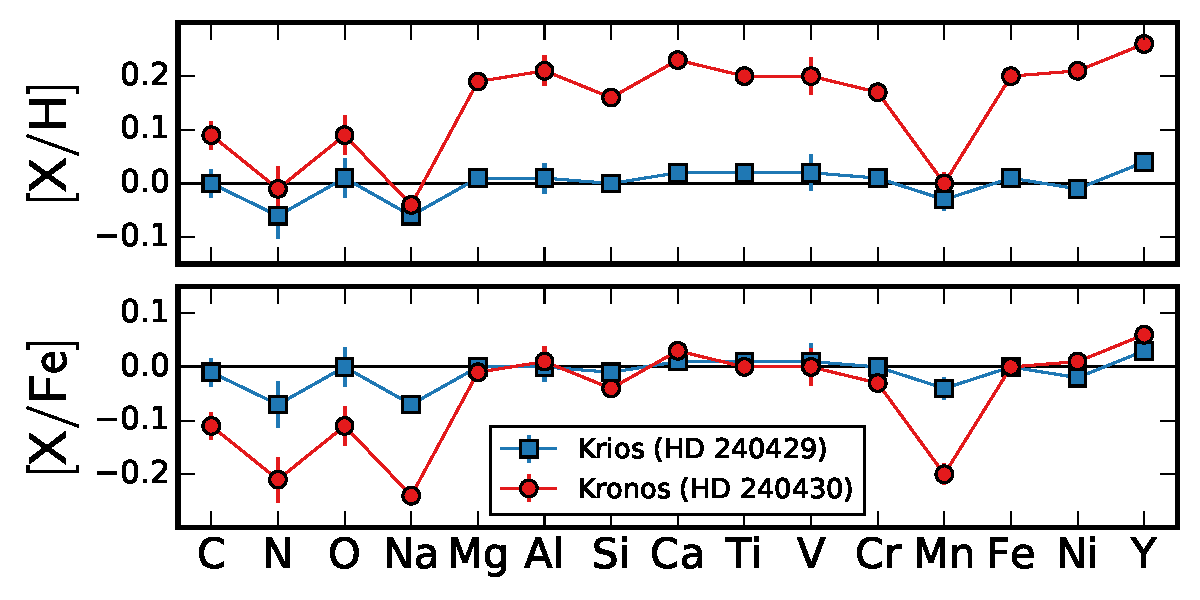
\includegraphics[width=0.9\linewidth]{abundances.pdf}
  \caption{Abundances of the comoving pair, \sunanalog\ and \bizarreone,
    normalized to \elem{H} (top) and \elem{Fe} (bottom).
    Lines are drawn for each star only to guide the eye.
    \bizarreone\ is enhanced in \elem{Fe} by $\approx 0.2$~dex relative to
    \sunanalog\ along with \elem{Mg}, \elem{Al}, \elem{Si}, \elem{Ca},
    \elem{Ti}, \elem{V}, \elem{Cr}, \elem{Ni}, \elem{Y} yet not in \elem{C},
    \elem{N}, \elem{O}, \elem{Na}, and \elem{Mn}.
    \label{fig:abundances}
  }
\end{figure}

\begin{table*}[htpb]
  \caption{Astrometric and spectroscopic measurements.}
  \label{tab:t1}
  \centering
  \begin{tabular}{ccc}
\hline\hline
Name & HD 240429 & HD 240430 \\
\hline
Sp Type                                   & G2                & G0                \\
$T_\mathrm{eff}$                          & 5878              & 5803              \\
$\log{g}$                                 & 4.43              & 4.33              \\
$v\sin{i}$                                & 1.1               & 2.5               \\
$[\elem{Fe}/\elem{H}]$                    & 0.01              & 0.20              \\
$v_r$                                     & $-21.2$           & $-21.2$           \\
$\varpi$ \footnotemark[1]                 & $9.35 \pm 0.24$   & $9.41 \pm 0.25$   \\
$\mu_\alpha^*$ \footnotemark[1]           & $89.25 \pm 0.66$  & $89.41 \pm 0.69$  \\
$\mu_\delta$ \footnotemark[1]             & $-29.68 \pm 0.54$ & $-30.12 \pm 0.52$ \\
\hline\hline 
\end{tabular}
\end{table*}

\sunanalog\ and \bizarreone\ were identified as a
candidate comoving star pair in our recent search for comoving stars using the
proper motions and parallaxes from the {\it Tycho-Gaia Astrometric Solution} catalog (hereafter \tgas),
a component of the astrometric space mission \gaia\ first data release
(the astrometric measurements are listed in \tablename~\ref{tab:t1}).
The pair has also been previously recognized as a visual double star system
in Washington Double Star catalog\cite{2001AJ....122.3466M}.
The two stars have spectral types G0 and G2 like the Sun.
In a separate effort to to study detailed chemical abundances of potential
planet-hosting stars, high resolution, high
signal-to-noise ratio spectra of both stars were obtained using the HIRES
spectrograph on the Keck-I telescope\cite{2016ApJS..225...32B}. 
The spectral resolution is $R=\lambda/\Delta\lambda\approx 70000$ and the
wavelength coverage is $5164$--$7799$~\AA.
A typical signal-to-noise ratio in the spectral continuum is $>200$~per pixel.
The resulting measurements include elemental abundances for 15 chemical species
(C, N, O, Na, Mg, Al, Si, Ca, Ti, V, Cr, Mn, Fe, Ni, Y) as well as stellar parameters
and high precision radial velocities.

The projected separation between the pair is 1.9 arcmin\ ($\approx 0.01$~pc),
and the 3D separation is $\approx 0.6$~pc.
Although selected based only on their astrometry, the two stars
have identical radial velocities within uncertainties (Table~\ref{tab:t1}),
confirming that they are truly comoving.
Combining these precise radial velocities with the \tgas\ astrometry, we
can compare differences between the inferred 6D phase-space coordinates of the
two stars.
For a 2~\msun\ binary system, the Jacobi radius in the Galactic neighborhood is
1.2~pc\cite{Jiang:2010aa}.
%TODO
\bizarreone\ and \sunanalog\ are likely a bound system that formed coevally.

%% abundance notation 
%We use the following convention for chemical abundances of stars: \elemH{X} is
%the log ratio of number density of element \elem{X} to \elem{H} relative to the
%solar value.
%The absolute abundance of \elem{X} is $A(\elem{X}) = 12 + \log_{10}
%(n_\elem{X}/n_\elem{H})$ where $n_\elem{X}$ is the number density of element
%\elem{X}.


Thus, we expect the two stars to have identical metallicities and abundance patterns.
However, one of the stars, \bizarreone\ is significantly more metal
rich than the other (by 0.2~dex $\approx 60\%$; \figname~\ref{fig:abundances}).
Moreover, not all elements are equally enhanced:
the abundances of \bizarreone\ show selective depletion in
\elem{C}, \elem{N}, \elem{O}, \elem{Na}, and \elem{Mn}
relative to \elem{Fe}.

The validity of the measured abundance differences is further demonstrated
in \figname~\ref{fig:spec1} and \ref{fig:spec2} where we show
segments of the spectra and models of the two stars
used to measure their abundances.
As expected from their reported metallicity difference ($\Delta\feh \approx 0.2$),
the ratio of data and model between the two stars show significant
residuals of almost all metal line features, largely dominated by \elem{Fe}.
However, for lines of elements that are not as enhanced in \bizarreone\,
the residuals are much smaller in amplitude.
%Li?

Assuming that the two stars were born together, one possibility to
explain the chemical difference is that there was chemical inhomogeneity within
the birth cloud.
However, there is already ample evidence against such a scenario.
First, none of the other seven similar wide binaries examined in
\cite{2016ApJS..225...32B} show the same level of differences in abundances.
Though there is generally a larger spread in $\elem{C}$, $\elem{N}$ and
$\elem{O}$, and some pairs show a difference in particular elements as large as
$\approx 0.15$~dex.
The median and maximum \feh\ difference between component stars in the other
seven pairs is $0.02$~dex and $0.09$~dex, respectively.
The differences are even smaller (maximum $\Delta\feh = 0.03$~dex) if we
compare only twin-like ($\Delta T_\mathrm{eff} \lesssim 100$~K) pairs
(\figname~\ref{fig:deltaXH}).
This is consistent with the findings of \cite{Desidera:2004aa}, who examined
23 wide binaries of late F to K dwarfs, and found most pairs show a difference
in \feh\ less than $0.02$~dex and none larger than $0.07$~dex.
Similarly, \cite{Gratton:2001aa} found that four out of six equal mass
binaries have the same chemical composition with $\gtrsim 0.01$~dex
uncertainties.
Thus, a difference of $\approx 0.2$~dex seen in \bizarreone-\sunanalog\ pair is
not likely due to chemical inhomogeneity in the birth cloud.

We stress that none of the other four twin-like ($\Delta T_\mathrm{eff}
\lesssim 100$~K) wide binary pairs examined by \cite{2016ApJS..225...32B}
show discrepancies in abundances between the stars at this level.
As shown in \figname~\ref{fig:deltaXH},
the differences in other pairs for all elements except \elem{N} and \elem{O},
which are also the most uncertain (\tablename~\ref{tab:kk}),
are less than $0.05$~dex, making \bizarreone-\sunanalog\ pair a significant outlier.

The spectra of both stars 
The \elem{Li} doublet at $6707.6$~\AA\ --- clearly visible in both spectra (see
\figname~\ref{fig:spec2}) --- for this sample was investigated in a separate
work (\cite{jmlithium}).
Both stars have high surface \elem{Li} abundances, and the difference in
\elem{Li} abundance ($\approx 0.5$~dex) is the largest among all elements
measured.


The fact that the two stars share nearly identical space motion
at a separation of $< 1$~pc strongly supports that the pair is coeval.
We therefore consider other age indicators apart from their phase-space
coordinates to assess the ages and coevality of the two stars.
First, given the precise measurements of $\log(g)$ and $T_\mathrm{eff}$,
we can constrain the ages of the two stars by
comparing these values to theoretical isochrones.
We perform isochrone fitting to these values using the Yale-Yonsei model
isochrones\cite{2013ApJ...776...87S}.
The input data are $\log(g)$, $T_\mathrm{eff}$, \feh,
parallaxes, $B$-band magnitudes, and their errors.
The best-fit isochrone ages of \sunanalog\ and \bizarreone\ are
$4.00_{-1.56}^{+1.51}$~Gyr and $4.28_{-1.03}^{+1.11}$~Gyr, respectively,
consistent with them being coeval.

The surface lithium abundance in a sun-like star decreases with its age due to
mixing induced by convection or rotation, which brings the lithium into the
interior ($T>2.5 \times 10^{6}$~K) where it will be destroyed by proton capture
burning.
Thus, surface lithium abundance is an indicator of stellar ages.
The absolute $\elem{Li}$ abundance of $2.25$~dex for \sunanalog\ implies an age
of $\lesssim 1$~Gyr according to the theoretical models tuned to explain the
solar lithium abundance and rotational profile (\cite{2005Sci...309.2189C}).
The lithium abundance of \bizarreone\, $2.74$~dex, shows the largest difference
among all measured elements.
This translates to a $\sim 500$~Myr difference in age.
Given the overall higher metal abundances and the peculiar abundance patterns
in \bizarreone, it is unclear, however, whether this higher $\elem{Li}$
abundance means a younger age or something else.
For example, the presence of $\elem{Li}$-rich red giant stars has been
attributed to the engulfment of substellar companions such as gas giant planets
or brown dwarfs which may replenish $\elem{Li}$ (\cite{Casey:2016aa}).

In fact, the surface lithium abundance is the only indication that points to
younger ages.
If the two stars are indeed only several hundred Myrs old at most,
they are expected to be part of a larger comoving group of stars.
However, as we mention above, there is no evidence in our search of comoving pairs
using \tgas\ that the two stars belong to a larger group of young stars.
Very young stars often show signs of activity such as
X-ray emission from magnetic activity, emission lines, or infrared excess due to
circumstellar disks (\todo{needs refernces}).
We have compiled GALEX, Tycho-2, 2MASS, and WISE photometry for these stars,
and found no evidence for indications of activity in their spectral energy
distributions.
The low $v\sin(i)$ values (\tablename~\ref{tab:kk}) also argue against very
young ages that would be inferred from the surface lithium abundances.
Finally, we computed the Galactic orbit of the pair using the median of the
posterior sample over the phase space coordinates of \sunanalog, in a Milky
Way-like gravitational potential (similar to \texttt{MWPotential2014} from
\cite{Bovy:2015}) using \project{Gala} (\cite{gala}).
The pair's fiducial orbit has a vertical action larger than the Sun, favoring
an older age (\todo{needs references for vertical action as age indicator}).
We therefore conclude that the two stars are most likely coeval, $\sim 4$~Gyr
old main sequence stars, and that their unusually high \elem{Li} abundance
requires an alternative explanation.


\begin{figure}[htpb]
  \centering
  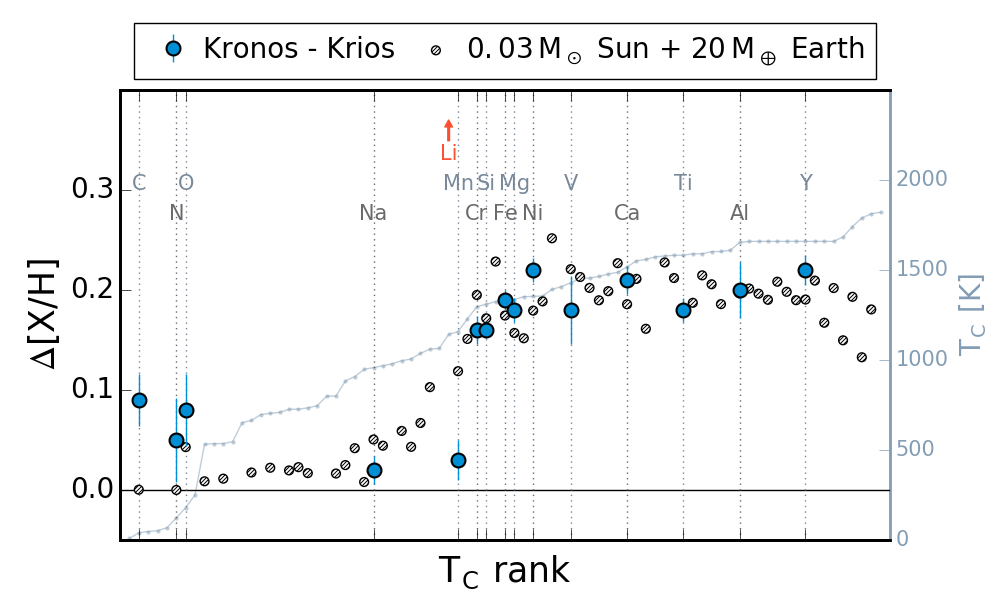
\includegraphics[width=0.95\linewidth]{toycalc.png}
  \caption{
    Comparing the observed abundance difference vs. \Tcondens\ rank
    to the expected change in solar surface abundance after adding $20$~\mearth\ of
    material with bulk Earth composition (\cite{mcdonough2001composition}).
    The assumed mass fraction in the convective zone is $0.03$.
    All metals are ranked by their \Tcondens\ for solar composition gas,
    and the condensation temperature may be read from the gray line and right y-axis,
    same as in \figname~\ref{fig:relabun_tcrank}.
    Locations of the elements measured for \bizarreone-\sunanalog\ pair are
    indicated by a vertical line and its symbol.
    The close match with the observed abundance difference in \bizarreone-\sunanalog\ pair
    suggests that the abundance difference may be due to accretion of
    $20$~\mearth\ of rocky planetary material.
    The element \elem{Li} is off the plot and indicated with a red arrow
    (see text for details).
  }
  \label{fig:toycalc}
\end{figure}


In Figure~\ref{fig:relabun_tcrank}, we show the abundance difference
between \bizarreone\ and \sunanalog\ ordered by the rank of \Tcondens\
of each element.
The equilibrium condensation temperatures for the composition of solar system
are taken from \cite{2003ApJ...591.1220L} (Table~8).
The difference seen in \bizarreone-\sunanalog\ is
compared to HD~20781/2, XO-2N/S, WASP-94A/B in \figname~\ref{fig:relabun_tcrank}.
The metallicity difference of $\approx 0.2$~dex observed in this pair
is larger than the differences seen in any other pairs studied so far.
Strikingly, the five under-enhanced elements in \bizarreone\
relative to \sunanalog\ are the five most volatile in all elements measured.
The difference in \elem{Mn} ($\Tcondens = 1158$~K) and
\elem{Cr} ($\Tcondens = 1296$~K) suggests a break in $\Tcondens \approx 1200$~K.
This $\Tcondens$-dependent trend of $\Delta\elemH{X}$,
combined with the enhanced $\elem{Li}$ abundance ($A(\elem{Li}) = 2.75$),
strongly suggests that accretion of rocky material has occured in \bizarreone.

We interpret the condensation temperature dependent
difference of elemental abundance between the two stars
as evidence for accretion of rocky planetary material in \bizarreone.
Instabilities may develop in a multi-planet system due to its chaotic nature
which may lead to planet engulfment or ejection by the host star
(\todo{needs references}).
%TODO: kozai?


One approach that is free from confusion with Galactic chemical evolution
is to compare two almost identical stars in a wide binary system.
Assuming that the component stars were born together with identical
initial composition, we may see a difference in their surface abundances
if the two stars then accreted different amounts of planetary material.
The resulting abundance difference may depend on the condensation
temperatures of elements in the protoplanetary disks from which the accreted
planets formed, as their compositions depend on the radial temperature gradient
in the disk.
%TODO: cautions on condensation temperature
% 1. it is just a proxy
% 2. it is **equlibrium** condensation temperature


How much mass of rocky material is needed to explain an increment of
$\approx 0.2$~dex?
We carry out simple toy calculations of expected $\Delta\elemH{X}$
in a Sun-like star's atmosphere by adding certain mass of bulk Earth composition
under these simplifying assumptions:
\begin{itemize}
  \item The material added is instantly and completely mixed.
  \item The atmospheric composition that we measure is identical throughout
    the star's radiative and convective zone.
  \item The surface abundance of the star has been altered only by the
    accretion event(s).
\end{itemize}
We take the solar abundances, $\elemH{X}$, of element \elem{X}
(\cite{Asplund:2009aa}) which can be converted to mass fraction as
\begin{equation}
  f_{X,\mathrm{photo}} = \frac{10^{\elemH{X}} m_X}{\Sigma_X 10^{\elemH{X}} m_X}
\end{equation}
where $m_X$ is the mass of each element in e.g., atomic mass unit.
Assuming that the added material has a total mass $M_\mathrm{add}$, and the
mass fraction in each element $f_{X,\mathrm{add}}$,
the abundance difference is
\begin{equation}
  \Delta\elemH{X} = \log_{10} \frac{f_{X,\mathrm{photo}}\,f_\mathrm{CZ}\,M_\mathrm{star}
    + f_{X,\mathrm{add}}\,M_\mathrm{add}}
    {f_{X,\mathrm{photo}}\,f_\mathrm{CZ}\,M_\mathrm{star}}
\end{equation}
where $f_\mathrm{CZ}$ is the fraction of the star's mass in the convective envelope.
We take the composition of bulk Earth from a chondritic model of the Earth
(\cite{mcdonough2001composition}).
Similar calculations have been performed by \citet{Chambers:2010aa} and
\citet{Mack:2014aa,Mack:2016aa}.

Figure~\ref{fig:toycalc} shows the expected change of surface abundances of
metals in a Sun-like star after $20~\mearth$ of material with composition of
bulk Earth is added.
A volatility trend that more volatile (low \Tcondens) elements are more
depleted in the Earth relative to CI or other carbonaceous chondrites
has long been known (\cite{mcdonough2001composition}).
This trend is presumed to be closely related to the formation of terrestrial
planets and, in particular to the radial temperature gradient in a
protoplanetary disk.
The trend resulting from adding $20~\mearth$ of bulk Earth
provides an overall good match to the observed $\Delta\elemH{X}$,
suggesting that the refractory-enhanced star, \bizarreone\,
accreted $20~\mearth$ more of rocky planetary material than \sunanalog.

What about \elem{Li}?
The element \elem{Li} is worth special attention in the context of the
accretion scenario.
Because Li is present in either carbonaceous chondrites or bulk Earth with
a concentration of $1-1.5$~ppm in mass (\cite{mcdonough2001composition}),
but is depleted quickly within the first couple of Gyrs on the surface of a
Sun-like star, accretion of either material at later times will significantly
replenish the lithium on the star's surface.
For the present-day Sun, the accretion of $20~\mearth$ of bulk Earth-like
material would result in $\Delta\elemH{Li} \approx 1.6$~dex (which
is indicated as an upward arrow in \figname~\ref{fig:toycalc}).
Incidentally, the star under examination, \bizarreone, has an age (informed by
stellar parameters) very close to the Sun ($4.28_{-1.03}^{+1.11}$~Gyr).
Thus, as long as we believe the Sun's present-day surface \elem{Li} abundance
to be ordinary, the accretion of $20$~\mearth\ by \bizarreone\ is consistent with $1.6$~dex
enhancement in its \elem{Li}.
This is exactly what we find: the \elem{Li} abundance of \bizarreone\ is
$A(\elem{Li}) = 2.75$ (Table~\ref{tab:kk}, \cite{jmlithium})
approximately $1.65$~dex higher than the solar value of $1.1$~dex
(\todo{needs reference}).
Furthermore, this implies that the accretion event should have happened very
recently, or at least within the \elem{Li} depletion time ($\lesssim 1$~Gyr).

What about \sunanalog?
Considering its age of $4.00_{-1.56}^{+1.51}$~Gyr, \sunanalog\ is also enhanced
in \elem{Li} compared to other stars of similar ages by $\approx 1$~dex.
This enhancement puts an upper limit on the accreted mass to be
$\approx 4$~\mearth\ assuming \elem{Li} concentration of $1.1$~ppm
(\cite{mcdonough2001composition}).
Unlike \bizarreone, we cannot know the pre-accretion abundances of
\sunanalog.\footnote{
  Strictly speaking, we can never know the pre-accretion abundances
  for \bizarreone\ either.
  We only have an {\it approximate} idea that this is not far from a solar-twin
  star \sunanalog, and because the deviation from this ``anchor'' star is
  large, it is reasonable to consider accretion by the Sun.
  In reality, \sunanalog\ may as well have had its own accretion history,
  which indeed seems to be the case according to its \elem{Li} abundance.
}
However, we note that the span of abundance difference between highly volatile
elements (\elem{C}, \elem{N}, \elem{O}, \elem{Na}) and refractory elements such
as \elem{Fe} expected from accreting $4$~\mearth\ to the Sun is $\approx
0.05$~dex.
This is comparable to the abundance difference between N, Na and Fe in
\sunanalog.
It is also interesting that \sunanalog\ shows a deficit in the same volatile
and moderately volatile elements (\elem{C}, \elem{N}, \elem{O}, \elem{Na}, and
\elem{Mn}) relative to Fe as in \bizarreone.
Thus, we conclude that \sunanalog\ is also likely to have had a similar
accretion event, but the amount of accretion was at least 5 time
smaller than \bizarreone.

%TODO: augment this paragraph
% - more geochemical study references
We stress that while the calculation carried out is useful in
an order-of-magnitude sense, further investigation of each of the simplifying
assumptions made is warranted.
In addition, the composition of bulk Earth has some uncertainties.
For example, the reported bulk Earth concentration of the siderphile element
\elem{Mn}, varies from $800$ to $1700$~ppm (\cite{1998psc..book.....L}).
While the latter value from \cite{mcdonough2001composition} has been used in
our calculation, the former value would bring the observed $\Delta\elemH{Mn}$
to an even closer agreement.
Given these limitations, the level of agreement for $\Delta\elemH{X}$ {\it and}
\elem{Li} for \bizarreone\ is remarkable.

Given that the two stars must have engulfed planets,
it is likely that they have not destroyed all of their planets.
Any surviving planet around the stars must be giants.
Fortunately, discovery of giant eccentric planets using astrometric jitter is in the sweet spot
for Gaia.
The two stars have not been included in any publicly released data from planet
search programs.
If both stars have accreted planetary material, it would be very interesting to
search for the existence and architectures of the planetary systems left
behind.


%\software{
%  %The data and code used in this project is available from
%  %\url{https://github.com/smoh/KronosKrios} under the MIT open-source
%  %software license.
%  This research utilized:
%  \texttt{Astropy} (\citealt{Astropy-Collaboration:2013}),
%  \texttt{emcee} (\citealt{2013PASP..125..306F}),
%  \texttt{IPython} (\citealt{Perez:2007}),
%  \texttt{matplotlib} (\citealt{Hunter:2007}),
%  \texttt{numpy} (\citealt{Van-der-Walt:2011}),
%  and \texttt{pandas} (\citealt{pandas}).}

\bibliography{ref}

\section*{Acknowledgements}
We thank Megan Bedell, Andy Casey, Keith Hawkins, Nathan Leigh, and Josh Winn
for feedback.
The Flatiron Institute is supported by the Simons Foundation.
% Gaia
This work has made use of data from the European Space Agency (ESA) mission
{\it Gaia} (\url{http://www.cosmos.esa.int/gaia}), processed by the {\it Gaia}
Data Processing and Analysis Consortium (DPAC,
\url{http://www.cosmos.esa.int/web/gaia/dpac/consortium}). Funding for the DPAC
has been provided by national institutions, in particular the institutions
participating in the {\it Gaia} Multilateral Agreement.

\section*{Extended Data}

\begin{table*}[htpb]
  \caption{Astrometric and spectroscopic measurements.}
  \label{tab:t2}
  \centering
  \begin{tabular}{ccc}
\hline\hline
Name & HD 240429 & HD 240430 \\
\hline
Sp Type                                   & G2                & G0                \\
$T_\mathrm{eff}$                          & 5878              & 5803              \\
$\log{g}$                                 & 4.43              & 4.33              \\
$v\sin{i}$                                & 1.1               & 2.5               \\
$[\elem{Fe}/\elem{H}]$                    & 0.01              & 0.20              \\
$v_r$                                     & $-21.2$           & $-21.2$           \\
$\varpi$ \footnotemark[1]                 & $9.35 \pm 0.24$   & $9.41 \pm 0.25$   \\
$\mu_\alpha^*$ \footnotemark[1]           & $89.25 \pm 0.66$  & $89.41 \pm 0.69$  \\
$\mu_\delta$ \footnotemark[1]             & $-29.68 \pm 0.54$ & $-30.12 \pm 0.52$ \\
\hline
\multicolumn{3}{c}{$T_c < 1200$~K} \\
\hline
$A(\elem{Li})$ \footnotemark[2]           & $2.25$            & $2.75$            \\
$\elemH{C}$                               & $0.00$            & $0.09$            \\
$\elemH{N}$                               & $-0.06$           & $-0.01$           \\
$\elemH{O}$                               & $0.01$            & $0.09$            \\
$\elemH{Na}$                              & $-0.06$           & $-0.04$           \\
$\elemH{Mn}$                              & $-0.03$           & $0.00$            \\
\hline
\multicolumn{3}{c}{$T_c > 1200$~K} \\
\hline
$\elemH{Mg}$                              & $0.01$            & $0.19$            \\
$\elemH{Al}$                              & $0.01$            & $0.21$            \\
$\elemH{Si}$                              & $0.00$            & $0.16$            \\
$\elemH{Ca}$                              & $0.02$            & $0.23$            \\
$\elemH{Ti}$                              & $0.02$            & $0.20$            \\
$\elemH{V}$                               & $0.02$            & $0.20$            \\
$\elemH{Cr}$                              & $0.01$            & $0.17$            \\
$\elemH{Fe}$                              & $0.01$            & $0.20$            \\
$\elemH{Ni}$                              & $-0.01$           & $0.21$            \\
$\elemH{Y}$                               & $0.04$            & $0.26$            \\
\hline\hline
\end{tabular}
%
%\begin{tablenotes}
%  \item All spectroscopic measurements except $\elem{Li}$ are from \citealt{2016ApJS..225...32B}.
%  \footnotetext[1]{From \tgas. }
%  \footnotetext[2]{Absolute abundance from \todo{CITE}.}
%\end{tablenotes}
\end{table*}

- all of table 1 here
- FIG: posterior of dx dv
- FIG: spectra + model
- FIG: orbits
- FIG: violin plot
- FIG: comparison to other pairs


\section*{Supplementary Information}


%\begin{deluxetable*}{c|cccc}
  \tablecaption{Astrometric and spectroscopic measurements of the pair
  \label{tab:kk}}
\tablehead{
  \colhead{}     & \colhead{}      & \sunanalog\         & \bizarreone\        & \colhead{} \\
  \colhead{Name} & \colhead{Units} & \colhead{HD 240429} & \colhead{HD 240430} & \colhead{Uncertainties}
}
\startdata
Sp Type                             &                & G0                     & G2                     &       \\
R.A.\tablenotemark{a}               & hh:mm:ss       & 23:51:55.21            & 23:52:09.42            &       \\
Dec.\tablenotemark{a}               & dd:mm:ss       & 59:42:48.16            &  59:42:26.08           &       \\
2MASS $J$\tablenotemark{a}          & mag            & $8.593 \pm 0.023$      & $8.415 \pm 0.026$      &       \\
$T_\mathrm{eff}$                    & K              & 5878                   & 5803                   & 25    \\
$\log{g}$                           &                & 4.43                   & 4.33                   & 0.028 \\
$v\sin{i}$                          & \kms\          & 1.1                    & 2.5                    &       \\
$[\elem{Fe}/\elem{H}]$              &                & 0.01                   & 0.20                   & 0.010 \\
Age\tablenotemark{b}                & Gyr            & $4.00_{-1.56}^{+1.51}$ & $4.28_{-1.03}^{+1.11}$ &       \\
$v_r$                               & \kms\          & $-21.2$                & $-21.2$                & 0.2   \\
$\varpi$\tablenotemark{a}          & mas            & $9.35 \pm 0.24$        & $9.41 \pm 0.25$        &       \\
$\mu_\alpha^*$\tablenotemark{a}    & mas\,yr$^{-1}$ & $89.25 \pm 0.66$       & $89.41 \pm 0.69$       &       \\
$\mu_\delta$\tablenotemark{a}      & mas\,yr$^{-1}$ & $-29.68 \pm 0.54$      & $-30.12 \pm 0.52$      &       \\
\hline
\multicolumn{5}{c}{$T_c < 1200$~K} \\
\hline
$A(\elem{Li})$\tablenotemark{c}    &                & $2.25$                 & $2.75$                 &       \\
$\elemH{C}$                         &                & $0.00$                 & $0.09$                 & 0.026 \\
$\elemH{N}$                         &                & $-0.06$                & $-0.01$                & 0.042 \\
$\elemH{O}$                         &                & $0.01$                 & $0.09$                 & 0.036 \\
$\elemH{Na}$                        &                & $-0.06$                & $-0.04$                & 0.014 \\
$\elemH{Mn}$                        &                & $-0.03$                & $0.00$                 & 0.020 \\
\hline
\multicolumn{5}{c}{$T_c > 1200$~K} \\
\hline
$\elemH{Mg}$                        &                & $0.01$                 & $0.19$                 & 0.012 \\
$\elemH{Al}$                        &                & $0.01$                 & $0.21$                 & 0.028 \\
$\elemH{Si}$                        &                & $0.00$                 & $0.16$                 & 0.008 \\
$\elemH{Ca}$                        &                & $0.02$                 & $0.23$                 & 0.014 \\
$\elemH{Ti}$                        &                & $0.02$                 & $0.20$                 & 0.012 \\
$\elemH{V}$                         &                & $0.02$                 & $0.20$                 & 0.034 \\
$\elemH{Cr}$                        &                & $0.01$                 & $0.17$                 & 0.014 \\
$\elemH{Fe}$                        &                & $0.01$                 & $0.20$                 & 0.010 \\
$\elemH{Ni}$                        &                & $-0.01$                & $0.21$                 & 0.014 \\
$\elemH{Y}$                         &                & $0.04$                 & $0.26$                 & 0.030 \\
\enddata
\tablenotetext{a}{From \tgas.}
\tablenotetext{b}{Derived in this work by isochrone fitting
  using the Yale-Yonsei model isochrones (\citealt{2013ApJ...776...87S}).}
\tablenotetext{c}{Absolute abundances from \citealt{jmlithium}.}
\tablecomments{
  All values are from \citealt{2016ApJS..225...32B} unless otherwise noted.
  The microturbulence parameter is fixed at $0.85$~\kms\ (\citealt{2015ApJ...805..126B}).
}
\end{deluxetable*}


\end{document}
